% Options for packages loaded elsewhere
\PassOptionsToPackage{unicode}{hyperref}
\PassOptionsToPackage{hyphens}{url}
%
\documentclass[
]{article}
\title{Predicting the Cost of Hotel Booking in the United States}
\author{LAM-duh: Xuliang Deng, Leah Okamura, Megan Richards}
\date{Nov 15th, 2021}

\usepackage{amsmath,amssymb}
\usepackage{lmodern}
\usepackage{iftex}
\ifPDFTeX
  \usepackage[T1]{fontenc}
  \usepackage[utf8]{inputenc}
  \usepackage{textcomp} % provide euro and other symbols
\else % if luatex or xetex
  \usepackage{unicode-math}
  \defaultfontfeatures{Scale=MatchLowercase}
  \defaultfontfeatures[\rmfamily]{Ligatures=TeX,Scale=1}
\fi
% Use upquote if available, for straight quotes in verbatim environments
\IfFileExists{upquote.sty}{\usepackage{upquote}}{}
\IfFileExists{microtype.sty}{% use microtype if available
  \usepackage[]{microtype}
  \UseMicrotypeSet[protrusion]{basicmath} % disable protrusion for tt fonts
}{}
\makeatletter
\@ifundefined{KOMAClassName}{% if non-KOMA class
  \IfFileExists{parskip.sty}{%
    \usepackage{parskip}
  }{% else
    \setlength{\parindent}{0pt}
    \setlength{\parskip}{6pt plus 2pt minus 1pt}}
}{% if KOMA class
  \KOMAoptions{parskip=half}}
\makeatother
\usepackage{xcolor}
\IfFileExists{xurl.sty}{\usepackage{xurl}}{} % add URL line breaks if available
\IfFileExists{bookmark.sty}{\usepackage{bookmark}}{\usepackage{hyperref}}
\hypersetup{
  pdftitle={Predicting the Cost of Hotel Booking in the United States},
  pdfauthor={LAM-duh: Xuliang Deng, Leah Okamura, Megan Richards},
  hidelinks,
  pdfcreator={LaTeX via pandoc}}
\urlstyle{same} % disable monospaced font for URLs
\usepackage[margin=1in]{geometry}
\usepackage{color}
\usepackage{fancyvrb}
\newcommand{\VerbBar}{|}
\newcommand{\VERB}{\Verb[commandchars=\\\{\}]}
\DefineVerbatimEnvironment{Highlighting}{Verbatim}{commandchars=\\\{\}}
% Add ',fontsize=\small' for more characters per line
\usepackage{framed}
\definecolor{shadecolor}{RGB}{248,248,248}
\newenvironment{Shaded}{\begin{snugshade}}{\end{snugshade}}
\newcommand{\AlertTok}[1]{\textcolor[rgb]{0.94,0.16,0.16}{#1}}
\newcommand{\AnnotationTok}[1]{\textcolor[rgb]{0.56,0.35,0.01}{\textbf{\textit{#1}}}}
\newcommand{\AttributeTok}[1]{\textcolor[rgb]{0.77,0.63,0.00}{#1}}
\newcommand{\BaseNTok}[1]{\textcolor[rgb]{0.00,0.00,0.81}{#1}}
\newcommand{\BuiltInTok}[1]{#1}
\newcommand{\CharTok}[1]{\textcolor[rgb]{0.31,0.60,0.02}{#1}}
\newcommand{\CommentTok}[1]{\textcolor[rgb]{0.56,0.35,0.01}{\textit{#1}}}
\newcommand{\CommentVarTok}[1]{\textcolor[rgb]{0.56,0.35,0.01}{\textbf{\textit{#1}}}}
\newcommand{\ConstantTok}[1]{\textcolor[rgb]{0.00,0.00,0.00}{#1}}
\newcommand{\ControlFlowTok}[1]{\textcolor[rgb]{0.13,0.29,0.53}{\textbf{#1}}}
\newcommand{\DataTypeTok}[1]{\textcolor[rgb]{0.13,0.29,0.53}{#1}}
\newcommand{\DecValTok}[1]{\textcolor[rgb]{0.00,0.00,0.81}{#1}}
\newcommand{\DocumentationTok}[1]{\textcolor[rgb]{0.56,0.35,0.01}{\textbf{\textit{#1}}}}
\newcommand{\ErrorTok}[1]{\textcolor[rgb]{0.64,0.00,0.00}{\textbf{#1}}}
\newcommand{\ExtensionTok}[1]{#1}
\newcommand{\FloatTok}[1]{\textcolor[rgb]{0.00,0.00,0.81}{#1}}
\newcommand{\FunctionTok}[1]{\textcolor[rgb]{0.00,0.00,0.00}{#1}}
\newcommand{\ImportTok}[1]{#1}
\newcommand{\InformationTok}[1]{\textcolor[rgb]{0.56,0.35,0.01}{\textbf{\textit{#1}}}}
\newcommand{\KeywordTok}[1]{\textcolor[rgb]{0.13,0.29,0.53}{\textbf{#1}}}
\newcommand{\NormalTok}[1]{#1}
\newcommand{\OperatorTok}[1]{\textcolor[rgb]{0.81,0.36,0.00}{\textbf{#1}}}
\newcommand{\OtherTok}[1]{\textcolor[rgb]{0.56,0.35,0.01}{#1}}
\newcommand{\PreprocessorTok}[1]{\textcolor[rgb]{0.56,0.35,0.01}{\textit{#1}}}
\newcommand{\RegionMarkerTok}[1]{#1}
\newcommand{\SpecialCharTok}[1]{\textcolor[rgb]{0.00,0.00,0.00}{#1}}
\newcommand{\SpecialStringTok}[1]{\textcolor[rgb]{0.31,0.60,0.02}{#1}}
\newcommand{\StringTok}[1]{\textcolor[rgb]{0.31,0.60,0.02}{#1}}
\newcommand{\VariableTok}[1]{\textcolor[rgb]{0.00,0.00,0.00}{#1}}
\newcommand{\VerbatimStringTok}[1]{\textcolor[rgb]{0.31,0.60,0.02}{#1}}
\newcommand{\WarningTok}[1]{\textcolor[rgb]{0.56,0.35,0.01}{\textbf{\textit{#1}}}}
\usepackage{longtable,booktabs,array}
\usepackage{calc} % for calculating minipage widths
% Correct order of tables after \paragraph or \subparagraph
\usepackage{etoolbox}
\makeatletter
\patchcmd\longtable{\par}{\if@noskipsec\mbox{}\fi\par}{}{}
\makeatother
% Allow footnotes in longtable head/foot
\IfFileExists{footnotehyper.sty}{\usepackage{footnotehyper}}{\usepackage{footnote}}
\makesavenoteenv{longtable}
\usepackage{graphicx}
\makeatletter
\def\maxwidth{\ifdim\Gin@nat@width>\linewidth\linewidth\else\Gin@nat@width\fi}
\def\maxheight{\ifdim\Gin@nat@height>\textheight\textheight\else\Gin@nat@height\fi}
\makeatother
% Scale images if necessary, so that they will not overflow the page
% margins by default, and it is still possible to overwrite the defaults
% using explicit options in \includegraphics[width, height, ...]{}
\setkeys{Gin}{width=\maxwidth,height=\maxheight,keepaspectratio}
% Set default figure placement to htbp
\makeatletter
\def\fps@figure{htbp}
\makeatother
\setlength{\emergencystretch}{3em} % prevent overfull lines
\providecommand{\tightlist}{%
  \setlength{\itemsep}{0pt}\setlength{\parskip}{0pt}}
\setcounter{secnumdepth}{-\maxdimen} % remove section numbering
\ifLuaTeX
  \usepackage{selnolig}  % disable illegal ligatures
\fi

\begin{document}
\maketitle

\hypertarget{introduction}{%
\subsubsection{Introduction}\label{introduction}}

With the lifting of travel restrictions into the U.S.
(\url{https://www.nytimes.com/2021/09/22/travel/us-international-travel-vaccine.html})
through the implementation of new travel guidelines, we believe that
travel to the U.S. start to increase and look like as it did before the
pandemic. Therefore, with travel and tourism in the U.S. increasing, we
believe that the booking of hotels may start to increase as well. With
this assumption, with the slower return to travel and society pre covid,
we are interested in studying the characteristics of hotel room
reservations in the United States. Specifically, we are interested in
what relationship these characteristics have with the cost of a hotel.
Our general research question is: How do the characteristics of a hotel
booking affect the daily cost of a hotel stay in the United States? We
believe there will be several significant points of relevance for
understanding these relationships: understanding predictors of room cost
could be used to help identify where new hotels could be successfully
created, allow travelers to plan financially for future travel, allow
hotels to predict future profit, etc. In this report, we are looking to
use a variety of chosen models to understand the contributing factors to
hotel room price, as well as identify the strongest predictors in the
determining the avreage daily rate.

\hypertarget{data}{%
\subsubsection{Data}\label{data}}

The source of the dataset is Tiny Tuesday,
\url{https://github.com/rfordatascience/tidytuesday/blob/master/data/2020/2020-02-11/readme.md}.
This data set was originally collected from an open hotel booking demand
dataset from Antonio, Almeida and Nunes, 2019. The data collected from
hotels all around the world ranges from bookings in 2015 to 2017. It is
sourced from this study
\url{https://www.sciencedirect.com/science/article/pii/S2352340918315191\#f0010}.
Due to the dataset being over 100,000 observations, we have limited the
observations to be only hotels from the US. The general characteristics
being measured in the data are the different aspects of booking and
staying at a hotel. For example, out of the 32 variables, some of the
ones we find great interest in are hotel type, reserved room type,
assigned room type, company, meal, number of adults/children/babies, the
average daily rate or daily cost, and the reservation status. Therefore,
each observation is one booking/stay at a specific hotel in America and
all of its characteristics. Therefore, there can be multiple
observations from the same hotel and even on the same time range. The
full dataset dictionary can be found in the repository ReadMe.

\hypertarget{resesarch-question}{%
\subsubsection{Resesarch Question}\label{resesarch-question}}

To better understand the contributing factors to the daily rate of hotel
rooms in the U.S., we will build models to:

\begin{enumerate}
\def\labelenumi{\arabic{enumi})}
\tightlist
\item
  Evaluate the efficacy of this model to predict daily hotel room rates
\item
  Evaluate the statistical significance of each predictor, identifying
  the strongest contributing factors. We include the following variables
  in our analysis: hotel type, company, meal, number of
  adults/children/babies, the average daily rate or daily cost, and the
  reservation status.
\end{enumerate}

\hypertarget{exploratory-data-analysis}{%
\subsubsection{Exploratory data
analysis}\label{exploratory-data-analysis}}

\begin{Shaded}
\begin{Highlighting}[]
\NormalTok{hotels}\SpecialCharTok{$}\NormalTok{total\_stay\_length }\OtherTok{\textless{}{-}}\NormalTok{ hotels}\SpecialCharTok{$}\NormalTok{stays\_in\_week\_nights }\SpecialCharTok{+}\NormalTok{ hotels}\SpecialCharTok{$}\NormalTok{stays\_in\_weekend\_nights}
\end{Highlighting}
\end{Shaded}

\begin{Shaded}
\begin{Highlighting}[]
\FunctionTok{ggplot}\NormalTok{(}\AttributeTok{data =}\NormalTok{ hotels, }\FunctionTok{aes}\NormalTok{(}\AttributeTok{x =}\NormalTok{ adr)) }\SpecialCharTok{+}
  \FunctionTok{geom\_histogram}\NormalTok{() }\SpecialCharTok{+} 
  \FunctionTok{labs}\NormalTok{(}\AttributeTok{x =} \StringTok{"Price in US Dollars"}\NormalTok{,}
       \AttributeTok{y =} \StringTok{"Frequency"}\NormalTok{, }
       \AttributeTok{title =} \StringTok{"Distribution of Average Daily Rate (Cost) of Hotel Bookings"}\NormalTok{,}
       \AttributeTok{subtitle =} \StringTok{"Collected from Hotels in the U.S. from 2015{-}2017"}\NormalTok{)}
\end{Highlighting}
\end{Shaded}

\begin{verbatim}
## `stat_bin()` using `bins = 30`. Pick better value with `binwidth`.
\end{verbatim}

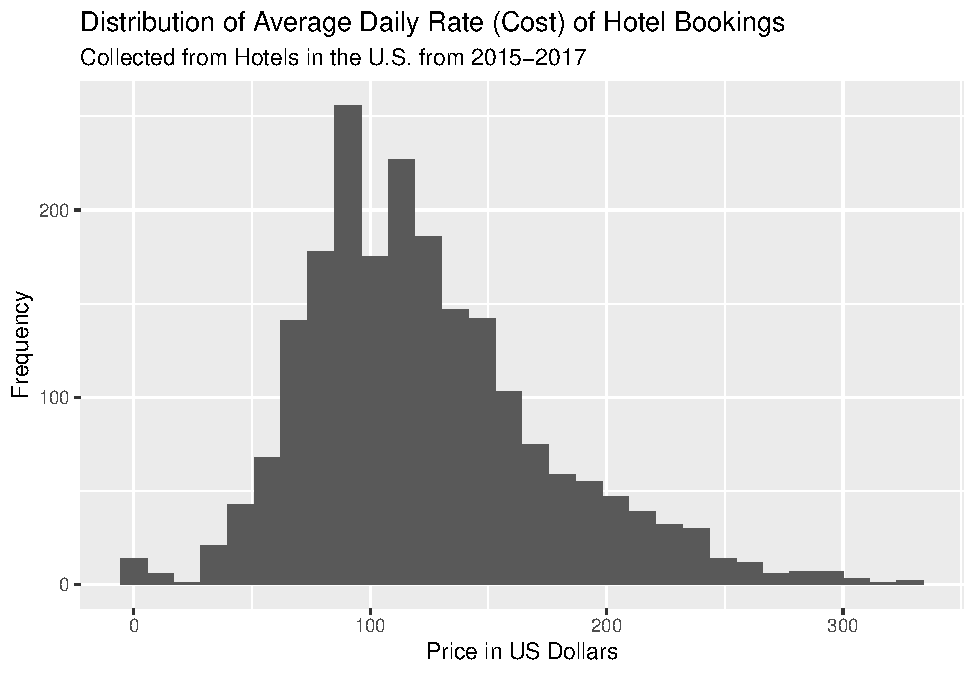
\includegraphics{written_report_files/figure-latex/response-plot-1.pdf}

\begin{Shaded}
\begin{Highlighting}[]
\NormalTok{hotels }\SpecialCharTok{\%\textgreater{}\%}
    \FunctionTok{summarise}\NormalTok{(}\AttributeTok{mean =} \FunctionTok{mean}\NormalTok{(adr), }
              \AttributeTok{median =} \FunctionTok{median}\NormalTok{(adr), }
              \AttributeTok{sd =} \FunctionTok{sd}\NormalTok{(adr),}
              \AttributeTok{min =} \FunctionTok{min}\NormalTok{(adr),}
              \AttributeTok{max =} \FunctionTok{max}\NormalTok{(adr),}
              \AttributeTok{iqr =} \FunctionTok{IQR}\NormalTok{(adr))}\SpecialCharTok{\%\textgreater{}\%}
\FunctionTok{kable}\NormalTok{(}\AttributeTok{digits =} \DecValTok{3}\NormalTok{)}
\end{Highlighting}
\end{Shaded}

\begin{longtable}[]{@{}rrrrrr@{}}
\toprule
mean & median & sd & min & max & iqr \\
\midrule
\endhead
122.992 & 115 & 51.617 & 0 & 328.33 & 61.99 \\
\bottomrule
\end{longtable}

The response variable, adr, has a somewhat skewed right, bimodal
distribution. The average or mean average daily rate is \$122.992 and
the median is \$115. Because the distribution is skewed, the median is
most likely the best indicator for the center. The standard deviation is
\$51.617 and the data ranges from \$0 to \$328.33 with an interquartile
range of \$61.99.

\begin{Shaded}
\begin{Highlighting}[]
\NormalTok{adults }\OtherTok{\textless{}{-}} \FunctionTok{sum}\NormalTok{(hotels}\SpecialCharTok{$}\NormalTok{adults)}
\NormalTok{children }\OtherTok{\textless{}{-}} \FunctionTok{sum}\NormalTok{(hotels}\SpecialCharTok{$}\NormalTok{children)}
\NormalTok{babies }\OtherTok{\textless{}{-}} \FunctionTok{sum}\NormalTok{(hotels}\SpecialCharTok{$}\NormalTok{babies)}

\NormalTok{tb }\OtherTok{\textless{}{-}} \FunctionTok{table}\NormalTok{(adults, children, babies)}
\FunctionTok{kable}\NormalTok{(tb)}
\end{Highlighting}
\end{Shaded}

\begin{longtable}[]{@{}lllr@{}}
\toprule
adults & children & babies & Freq \\
\midrule
\endhead
3950 & 362 & 6 & 1 \\
\bottomrule
\end{longtable}

This table provides insight on the type of people who were booking
hotels in the U.S. during this time period. A large majority of
customers were only adults with a total of 3,950 hotel bookings. The
next largest customer group were people or adults with their children at
a total of 362 bookings. Lastly, those who booked a stay with a baby was
considerably less, with only 6 bookings.

\begin{Shaded}
\begin{Highlighting}[]
\FunctionTok{ggplot}\NormalTok{(}\AttributeTok{data =}\NormalTok{ hotels, }\FunctionTok{aes}\NormalTok{(}\AttributeTok{x =}\NormalTok{ meal)) }\SpecialCharTok{+}
\FunctionTok{geom\_bar}\NormalTok{() }\SpecialCharTok{+}
\FunctionTok{labs}\NormalTok{(}\AttributeTok{title =} \StringTok{"Distribution of Meal Plan According to Booking Details"}\NormalTok{,}
      \AttributeTok{y =} \StringTok{"Frequency"}\NormalTok{,}
      \AttributeTok{x =} \StringTok{"Type of Meal Plan"}\NormalTok{) }
\end{Highlighting}
\end{Shaded}

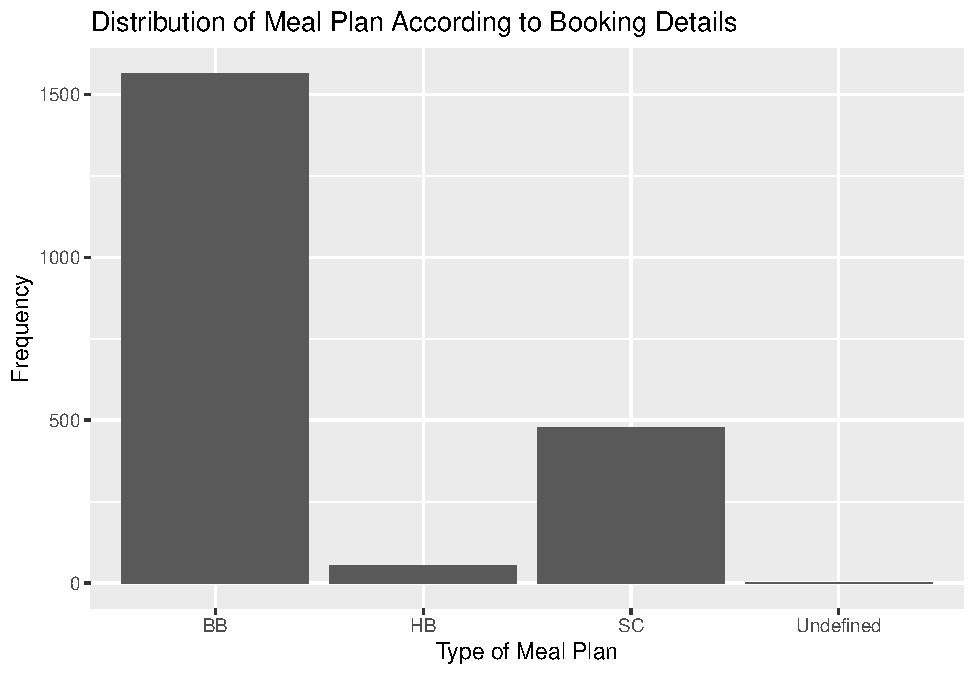
\includegraphics{written_report_files/figure-latex/unnamed-chunk-2-1.pdf}

\begin{Shaded}
\begin{Highlighting}[]
\NormalTok{hotels }\SpecialCharTok{\%\textgreater{}\%}
  \FunctionTok{group\_by}\NormalTok{(meal) }\SpecialCharTok{\%\textgreater{}\%}
  \FunctionTok{summarise}\NormalTok{(}\AttributeTok{n =} \FunctionTok{n}\NormalTok{(), }\AttributeTok{mean =} \FunctionTok{mean}\NormalTok{(adr), }\AttributeTok{sd =} \FunctionTok{sd}\NormalTok{(adr)) }\SpecialCharTok{\%\textgreater{}\%}
  \FunctionTok{kable}\NormalTok{(}\AttributeTok{digits =} \DecValTok{3}\NormalTok{)}
\end{Highlighting}
\end{Shaded}

\begin{longtable}[]{@{}lrrr@{}}
\toprule
meal & n & mean & sd \\
\midrule
\endhead
BB & 1563 & 127.834 & 54.168 \\
HB & 55 & 167.216 & 60.824 \\
SC & 478 & 101.678 & 29.128 \\
Undefined & 1 & 311.000 & NA \\
\bottomrule
\end{longtable}

We can see that majority of customer bookings chose the Bed and
Breakfast plan (BB), rather than Half Board plan or Full Board (HB and
SC). While this does reflect the choice of those booking the hotel, this
visualization and dataset can also be influenced by what type of meal
plan each hotel is offering.

\begin{Shaded}
\begin{Highlighting}[]
\FunctionTok{ggplot}\NormalTok{(}\AttributeTok{data =}\NormalTok{ hotels, }\FunctionTok{aes}\NormalTok{(}\AttributeTok{x =}\NormalTok{ reservation\_status)) }\SpecialCharTok{+}
\FunctionTok{geom\_bar}\NormalTok{() }\SpecialCharTok{+}
\FunctionTok{labs}\NormalTok{(}\AttributeTok{title =} \StringTok{"Distribution of Reservation Status"}\NormalTok{,}
  \AttributeTok{x =} \StringTok{"Type of Status"}\NormalTok{,}
  \AttributeTok{y =} \StringTok{"Frequency"}\NormalTok{) }
\end{Highlighting}
\end{Shaded}

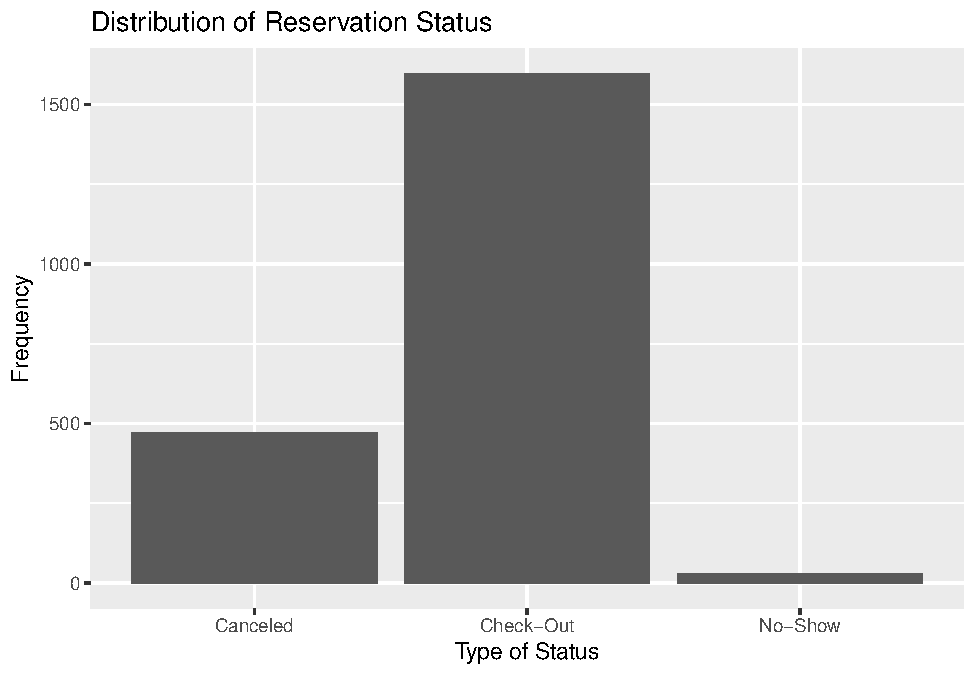
\includegraphics{written_report_files/figure-latex/unnamed-chunk-4-1.pdf}
A vast majority of the reservation statuses in this dataset resulted in
a check-out, meaning that the customer arrived and stayed for the
duration of the stay. It also important to note that a substantial
proportion of hotel bookings were canceled, and if possible we would
like to investigate what relationship might exist here.

\begin{Shaded}
\begin{Highlighting}[]
\NormalTok{hotels }\SpecialCharTok{\%\textgreater{}\%}
  \FunctionTok{group\_by}\NormalTok{(hotel) }\SpecialCharTok{\%\textgreater{}\%}
  \FunctionTok{summarise}\NormalTok{(}\AttributeTok{n =} \FunctionTok{n}\NormalTok{(), }\AttributeTok{mean =} \FunctionTok{mean}\NormalTok{(adr), }\AttributeTok{sd =} \FunctionTok{sd}\NormalTok{(adr)) }\SpecialCharTok{\%\textgreater{}\%}
  \FunctionTok{kable}\NormalTok{(}\AttributeTok{digits =} \DecValTok{3}\NormalTok{)}
\end{Highlighting}
\end{Shaded}

\begin{longtable}[]{@{}lrrr@{}}
\toprule
hotel & n & mean & sd \\
\midrule
\endhead
City Hotel & 1618 & 119.773 & 45.189 \\
Resort Hotel & 479 & 133.865 & 67.982 \\
\bottomrule
\end{longtable}

We can see that resort hotel is on average more expensive, and that most
customers booked at city hotels. We are interested in whether the
classification of City Hotel and Resort Hotel will proportionately have
similar relationships with the other variables.

\begin{Shaded}
\begin{Highlighting}[]
\FunctionTok{ggplot}\NormalTok{(}\AttributeTok{data =}\NormalTok{ hotels, }\FunctionTok{aes}\NormalTok{(}\AttributeTok{x =}\NormalTok{ lead\_time, }\AttributeTok{y =}\NormalTok{ adr, }\AttributeTok{color =}\NormalTok{ hotel)) }\SpecialCharTok{+}
\FunctionTok{geom\_point}\NormalTok{() }\SpecialCharTok{+}
\FunctionTok{labs}\NormalTok{(}\AttributeTok{title =} \StringTok{"Relationship between how early people book hotel and price in the US dollars"}\NormalTok{,}
  \AttributeTok{x =} \StringTok{"Subtraction of entering date from arrival date"}\NormalTok{,}
  \AttributeTok{y =} \StringTok{"Price in the US Dollars"}\NormalTok{) }
\end{Highlighting}
\end{Shaded}

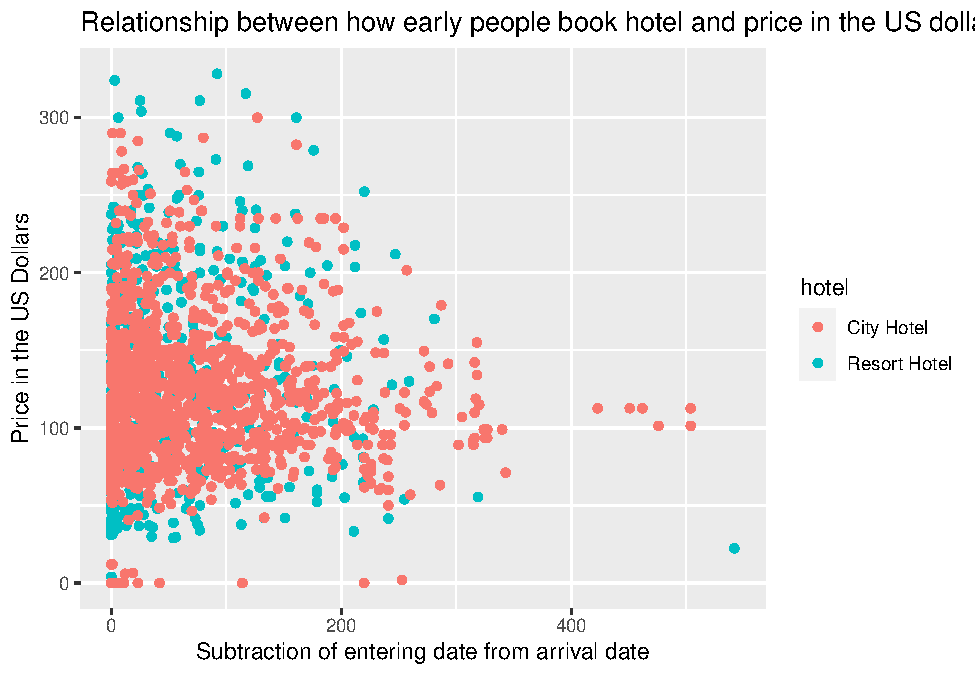
\includegraphics{written_report_files/figure-latex/unnamed-chunk-6-1.pdf}
We can see that the more last minute visitors book a hotel, the more
likely it is that the price in the US dollars varies. Besides, we can
also see that the highest price in a hotel decreases as the difference
between entering data and arrival date increases. This could suggest
that the earlier you book a hotel, the price is more likely to be cheap.

\begin{Shaded}
\begin{Highlighting}[]
\FunctionTok{ggplot}\NormalTok{(}\AttributeTok{data =}\NormalTok{ hotels, }\FunctionTok{aes}\NormalTok{(}\AttributeTok{x =}\NormalTok{ adr, }\AttributeTok{y =}\NormalTok{ arrival\_date\_day\_of\_month, }\AttributeTok{color=}\NormalTok{hotel)) }\SpecialCharTok{+}
\FunctionTok{geom\_point}\NormalTok{() }\SpecialCharTok{+}
\FunctionTok{labs}\NormalTok{(}\AttributeTok{title =} \StringTok{"Relationship between day in the month when hotels are booked and price in the US dollars"}\NormalTok{,}
  \AttributeTok{x =} \StringTok{"Day in the month"}\NormalTok{,}
  \AttributeTok{y =} \StringTok{"Price in US Dollars"}\NormalTok{) }
\end{Highlighting}
\end{Shaded}

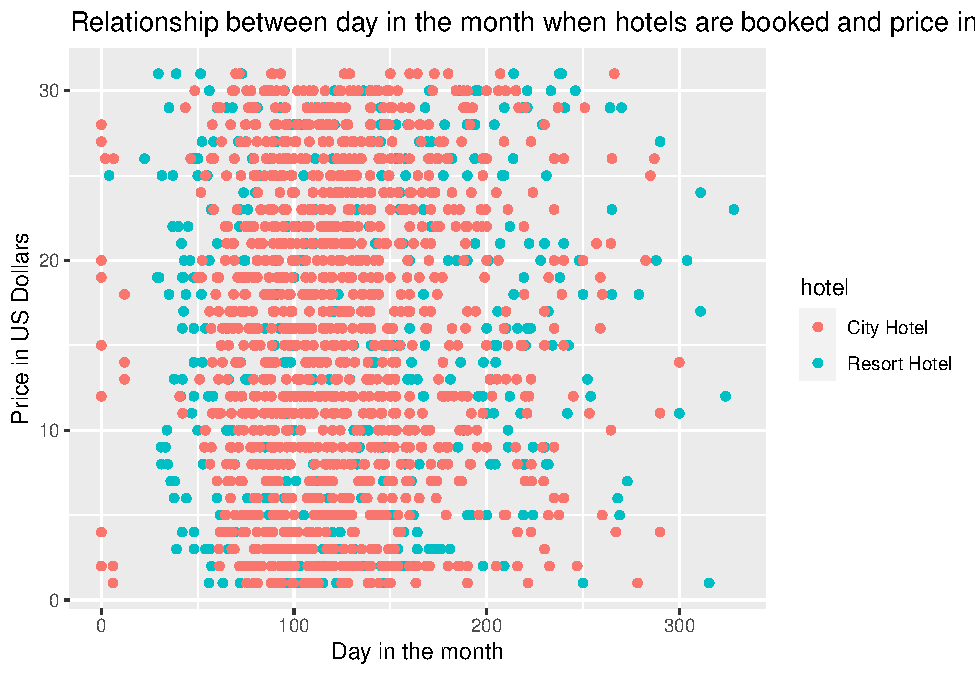
\includegraphics{written_report_files/figure-latex/unnamed-chunk-7-1.pdf}
We cannot see any significant relationship between day in the month and
the hotel price from this figure. However, we can see that summer is the
busiest season for hotels and the price varies evenly. At the beginning
of the year and the end of the year, hotels are not really booked as
often.

\begin{Shaded}
\begin{Highlighting}[]
\FunctionTok{ggplot}\NormalTok{(}\AttributeTok{data =}\NormalTok{ hotels, }\FunctionTok{aes}\NormalTok{(}\AttributeTok{x =}\NormalTok{ arrival\_date\_week\_number, }\AttributeTok{y =}\NormalTok{ adr, }\AttributeTok{color=}\NormalTok{hotel)) }\SpecialCharTok{+}
\FunctionTok{geom\_point}\NormalTok{() }\SpecialCharTok{+}
\FunctionTok{labs}\NormalTok{(}\AttributeTok{title =} \StringTok{"Relationship between week in the year when hotels are booked and price in the US dollars"}\NormalTok{,}
  \AttributeTok{x =} \StringTok{"Week in the year"}\NormalTok{,}
  \AttributeTok{y =} \StringTok{"Price in US Dollars"}\NormalTok{) }
\end{Highlighting}
\end{Shaded}

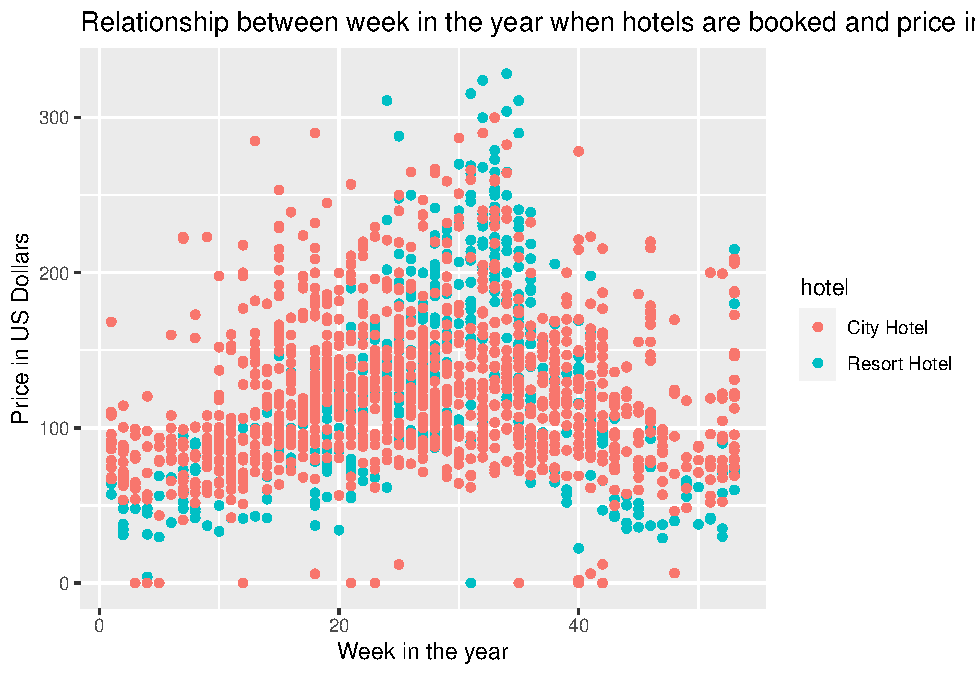
\includegraphics{written_report_files/figure-latex/unnamed-chunk-8-1.pdf}
From this figure, we can also see that at the beginning and end of the
year hotels are not as busy as during the summer. Besides, we can also
observe that the price of hotel tends to become higher during summer
time compared to the rest of the year.

We are particularly interested in using the hotel type (Resort versus
City Hotel) as a predictor of average daily rate. As an initial
analysis, we perform a t-test on the the average daily rates of bookings
for resort versus city hotels. This t-test assesses if there is a
significant difference between the two distributions, which would
indicate that hotel type is likely to be a useful predictor of average
daily rate. In this analysis, we find that our t-test produces a p-value
of 0.002305\%. Because this p-value is very low, we conclude that there
is a statistically significant relationship between the average daily
hotel rates of resort hotels and city hotels in our dataset, which
provides evidence that hotel type is a useful predictor of average daily
hotel rates.

\begin{Shaded}
\begin{Highlighting}[]
\NormalTok{resort\_adr }\OtherTok{\textless{}{-}}\NormalTok{ hotels[hotels}\SpecialCharTok{$}\NormalTok{hotel }\SpecialCharTok{==} \StringTok{"Resort Hotel"}\NormalTok{,]}\SpecialCharTok{$}\NormalTok{adr}
\NormalTok{city\_adr }\OtherTok{\textless{}{-}}\NormalTok{ hotels[hotels}\SpecialCharTok{$}\NormalTok{hotel }\SpecialCharTok{==} \StringTok{"City Hotel"}\NormalTok{,]}\SpecialCharTok{$}\NormalTok{adr}

\NormalTok{hotel\_type\_p\_value }\OtherTok{\textless{}{-}} \FunctionTok{t.test}\NormalTok{(resort\_adr, city\_adr)}\SpecialCharTok{$}\NormalTok{p.value}
\FunctionTok{print}\NormalTok{(hotel\_type\_p\_value)}
\end{Highlighting}
\end{Shaded}

\begin{verbatim}
## [1] 2.304792e-05
\end{verbatim}

We are also particularly interested in using the presence of kids
(children or babies) as a predictor of average daily rate. As an initial
analysis, we perform a t-test on the the average daily rates of bookings
for groups with only adults, versus groups with children or babies. This
t-test assesses if there is a significant difference between the two
distributions, which would indicate that the presence of kids is likely
to be a useful predictor of average daily rate. In this analysis, we
find that our t-test produces a p-value of 1.13e-33\%. Because this
p-value is very low, we conclude that there is a statistically
significant relationship between the average daily hotel rates of groups
with children or babies and groups with only adults in our dataset,
which provides evidence that the presence of kids (children or babies)
is a useful predictor of average daily hotel rates.

\begin{Shaded}
\begin{Highlighting}[]
\NormalTok{hotels}\SpecialCharTok{$}\NormalTok{only\_adults\_present }\OtherTok{\textless{}{-}}\NormalTok{ hotels}\SpecialCharTok{$}\NormalTok{adults }\SpecialCharTok{\textgreater{}} \DecValTok{0} \SpecialCharTok{\&}\NormalTok{ hotels}\SpecialCharTok{$}\NormalTok{children }\SpecialCharTok{==} \DecValTok{0} \SpecialCharTok{\&}\NormalTok{ hotels}\SpecialCharTok{$}\NormalTok{babies }\SpecialCharTok{==} \DecValTok{0}
\NormalTok{hotels}\SpecialCharTok{$}\NormalTok{kids\_present }\OtherTok{\textless{}{-}}\NormalTok{ hotels}\SpecialCharTok{$}\NormalTok{children }\SpecialCharTok{\textgreater{}} \DecValTok{0} \SpecialCharTok{|}\NormalTok{ hotels}\SpecialCharTok{$}\NormalTok{babies }\SpecialCharTok{\textgreater{}} \DecValTok{0}

\NormalTok{adult\_adr }\OtherTok{\textless{}{-}}\NormalTok{ hotels[hotels}\SpecialCharTok{$}\NormalTok{only\_adults\_present }\SpecialCharTok{==} \ConstantTok{TRUE}\NormalTok{,]}\SpecialCharTok{$}\NormalTok{adr}
\NormalTok{kids\_adr }\OtherTok{\textless{}{-}}\NormalTok{ hotels[hotels}\SpecialCharTok{$}\NormalTok{kids\_present }\SpecialCharTok{==} \ConstantTok{TRUE}\NormalTok{,]}\SpecialCharTok{$}\NormalTok{adr}

\NormalTok{resident\_type\_p\_value }\OtherTok{\textless{}{-}} \FunctionTok{t.test}\NormalTok{(adult\_adr, kids\_adr)}\SpecialCharTok{$}\NormalTok{p.value}
\FunctionTok{print}\NormalTok{(resident\_type\_p\_value)}
\end{Highlighting}
\end{Shaded}

\begin{verbatim}
## [1] 1.134618e-35
\end{verbatim}

\hypertarget{methodology}{%
\subsection{Methodology}\label{methodology}}

\hypertarget{modeling-choices-description}{%
\subsubsection{Modeling Choices
(Description)}\label{modeling-choices-description}}

\begin{itemize}
\tightlist
\item
  Data transformations (if applied)
\item
  Model Type Justification
\item
  Model selection criteria
\item
  Handling Interaction Terms
\item
  Any other technical choices
\end{itemize}

It is important to note that there are a few variables in the dataset
that do not provide insight to our research question and as a result we
will remove from the dataset. First is the category
\texttt{hotels\$country}, due to the fact that every hotel in this
subset of the data is located in the U.S., this is a redundant variable.
Next, the two variables \texttt{hotels\$reserved\_room\_type} and
\texttt{hotels\$assigned\_room\_type} are both categorical variables
that have letters assigned to each room type. However, due to the
confidentiality of the customers, the classification of these letters
have not been identified by those who collected the data. Therefore, we
will be removing these variables from the dataset.

\begin{Shaded}
\begin{Highlighting}[]
\NormalTok{hotels}\SpecialCharTok{$}\NormalTok{country }\OtherTok{\textless{}{-}} \ConstantTok{NULL} 
\NormalTok{hotels}\SpecialCharTok{$}\NormalTok{reserved\_room\_type }\OtherTok{\textless{}{-}} \ConstantTok{NULL} 
\NormalTok{hotels}\SpecialCharTok{$}\NormalTok{assigned\_room\_type }\OtherTok{\textless{}{-}} \ConstantTok{NULL} 
\end{Highlighting}
\end{Shaded}

As of now, we know we are going to use hotel (Resort Hotel or City
Hotel), company, customer\_type, stays\_in\_weekend\_nights,
stays\_in\_week\_nights, and meal(type of meal) as predictor variables.
We are interested in how the food is served at a hotel and what type of
hotel can indicate how much a night in a hotel could cost. As we explore
more of the relationships in our dataset, we may add other possible
predictor variables as we see fit.

We plan to use multiple linear regression with a variety of combinations
of interested predictor variables and their interaction. Based on
whether conditions or fit or not or based on the visualization, we
believe we may be utilizing logarithmic regression as well. We would
also be interested in seeing how stays in the weekend or the weekday may
affect the average daily rate for a hotel, and if they differ between
the two hotel types, City and Resort hotels.

\hypertarget{modeling}{%
\subsubsection{Modeling}\label{modeling}}

\begin{Shaded}
\begin{Highlighting}[]
\NormalTok{model }\OtherTok{\textless{}{-}} \FunctionTok{lm}\NormalTok{(adr }\SpecialCharTok{\textasciitilde{}}\NormalTok{ adults }\SpecialCharTok{+}\NormalTok{ children }\SpecialCharTok{+}\NormalTok{ babies }\SpecialCharTok{+}\NormalTok{ hotel }\SpecialCharTok{+}\NormalTok{ meal }\SpecialCharTok{+}\NormalTok{ reservation\_status, }\AttributeTok{data =}\NormalTok{ hotels)}
\end{Highlighting}
\end{Shaded}

\hypertarget{conditions-check-for-linear-model}{%
\subsubsection{Conditions Check For Linear
Model}\label{conditions-check-for-linear-model}}

\begin{Shaded}
\begin{Highlighting}[]
\CommentTok{\# Residual + QQ Plots}
\FunctionTok{autoplot}\NormalTok{(model, }\AttributeTok{which =} \FunctionTok{c}\NormalTok{(}\DecValTok{1}\NormalTok{,}\DecValTok{2}\NormalTok{))}
\end{Highlighting}
\end{Shaded}

\includegraphics{written_report_files/figure-latex/unnamed-chunk-11-1.pdf}
• Linearity The residuals are randomly scattered in the plot of
residuals vs fitted, so the linearity condition is satisfied. • Constant
variance: The spread of the residuals is approximately equal in the plot
of residuals vs.~fitted as the fitted value increases. There are a few
outliers, but overall the spread of the residuals is equal. Therefore
constant variance is satisfied. • Normality: The QQ-plot shows that the
distribution of the residuals is skewed right, so this condition is not
satisfied. However, the model is robust to deviations from normality for
sample sizes greater than 30. Our sample size of 1447 is greater than
30, so we can proceed. • Independence: This condition is not met since
there are multiple observations for most lemurs. These observations
would be correlated

From this analysis, we conclude that the conditions are met for
performing linear regression.

\hypertarget{results}{%
\subsection{Results}\label{results}}

\begin{Shaded}
\begin{Highlighting}[]
\FunctionTok{tidy}\NormalTok{(model, }\AttributeTok{conf.int =} \ConstantTok{TRUE}\NormalTok{) }\SpecialCharTok{\%\textgreater{}\%}
\FunctionTok{kable}\NormalTok{(}\AttributeTok{digits =} \DecValTok{3}\NormalTok{)}
\end{Highlighting}
\end{Shaded}

\begin{longtable}[]{@{}lrrrrrr@{}}
\toprule
term & estimate & std.error & statistic & p.value & conf.low &
conf.high \\
\midrule
\endhead
(Intercept) & 79.723 & 4.256 & 18.734 & 0.000 & 71.377 & 88.069 \\
adults & 26.277 & 1.825 & 14.398 & 0.000 & 22.698 & 29.856 \\
children & 35.169 & 1.825 & 19.274 & 0.000 & 31.590 & 38.747 \\
babies & -22.637 & 17.815 & -1.271 & 0.204 & -57.574 & 12.300 \\
hotelResort Hotel & 2.353 & 2.391 & 0.984 & 0.325 & -2.336 & 7.042 \\
mealHB & 33.779 & 5.982 & 5.647 & 0.000 & 22.048 & 45.511 \\
mealSC & -17.205 & 2.409 & -7.141 & 0.000 & -21.930 & -12.480 \\
mealUndefined & 106.033 & 43.632 & 2.430 & 0.015 & 20.466 & 191.600 \\
reservation\_statusCheck-Out & -12.809 & 2.323 & -5.515 & 0.000 &
-17.364 & -8.254 \\
reservation\_statusNo-Show & -2.662 & 8.327 & -0.320 & 0.749 & -18.991 &
13.668 \\
\bottomrule
\end{longtable}

\[\hat{Average Daily Rate} = 79.723  + 79.723   (adults) + 35.169(children)\]
\[ -22.637(babies) + 2.353(hotel Resort Hotel) + 33.779 (mealHB) - 17.205(mealSc)\]
\[+106.033(mealUndefined)-12.809(reservationstatusCheck-Out) - 2.662(reservationstatusNo-Show)\]

\hypertarget{diagnostics}{%
\subsubsection{Diagnostics}\label{diagnostics}}

\begin{Shaded}
\begin{Highlighting}[]
\FunctionTok{autoplot}\NormalTok{(model, }\AttributeTok{which =} \FunctionTok{c}\NormalTok{(}\DecValTok{3}\NormalTok{, }\DecValTok{4}\NormalTok{, }\DecValTok{5}\NormalTok{))}
\end{Highlighting}
\end{Shaded}

\begin{verbatim}
## Warning: Removed 14 row(s) containing missing values (geom_path).
\end{verbatim}

\begin{verbatim}
## Warning: Removed 1 rows containing missing values (geom_segment).
\end{verbatim}

\begin{verbatim}
## Warning: Removed 1 rows containing missing values (geom_point).
\end{verbatim}

\includegraphics{written_report_files/figure-latex/unnamed-chunk-12-1.pdf}

\begin{Shaded}
\begin{Highlighting}[]
\CommentTok{\#Leverage }
\NormalTok{lev\_threshold }\OtherTok{\textless{}{-}} \DecValTok{2} \SpecialCharTok{*} \DecValTok{2} \SpecialCharTok{/} \FunctionTok{nrow}\NormalTok{(hotels) }
\NormalTok{hotel\_aug }\OtherTok{\textless{}{-}} \FunctionTok{augment}\NormalTok{(model) }

\NormalTok{hotel\_aug }\SpecialCharTok{\%\textgreater{}\%}
\FunctionTok{filter}\NormalTok{(.hat }\SpecialCharTok{\textgreater{}}\NormalTok{ lev\_threshold) }\SpecialCharTok{\%\textgreater{}\%} \FunctionTok{nrow}\NormalTok{()}
\end{Highlighting}
\end{Shaded}

\begin{verbatim}
## [1] 1604
\end{verbatim}

\begin{Shaded}
\begin{Highlighting}[]
\CommentTok{\# High Magnitude Residual }
\NormalTok{hotel\_aug }\SpecialCharTok{\%\textgreater{}\%}
\FunctionTok{filter}\NormalTok{(.std.resid }\SpecialCharTok{\textless{}} \SpecialCharTok{{-}}\DecValTok{3} \SpecialCharTok{|}\NormalTok{ .std.resid }\SpecialCharTok{\textgreater{}} \DecValTok{3}\NormalTok{) }\SpecialCharTok{\%\textgreater{}\%} \FunctionTok{nrow}\NormalTok{()}
\end{Highlighting}
\end{Shaded}

\begin{verbatim}
## [1] 10
\end{verbatim}

\begin{Shaded}
\begin{Highlighting}[]
\CommentTok{\# Influential Point }
\NormalTok{hotel\_aug }\SpecialCharTok{\%\textgreater{}\%}
\FunctionTok{filter}\NormalTok{(.cooksd }\SpecialCharTok{\textgreater{}} \FloatTok{1.0}\NormalTok{) }\SpecialCharTok{\%\textgreater{}\%} \FunctionTok{nrow}\NormalTok{()}
\end{Highlighting}
\end{Shaded}

\begin{verbatim}
## [1] 0
\end{verbatim}

We use leverage and Cook's Distance to identify influential observations
in our dataset, and use standardized residuals to identify outliers.

Leverage is a measure of the distance between an observation's values of
the predictor variables and the average values of the predictor
variables for the entire data set. We define a high leverage point as
having a leverage greater than \$ 2(p+1) /n \$, where p is the number of
predictors and n is the number of observations. We find X observations
to be high leverage, and consider them to be potential influential
points.

Cook's distance is a composite measure of an observation's leverage and
standardized residual, and is used to identify influential points. An
observation is considered an influential point if it's Cook's distance
is greater than 1.0. We find X observations with a Cook's distance
greater than 1.0, and conclude that they are influential points.

Standardized residuals can be used to identify outliers, as observations
that have standardized residuals of large magnitude don't fit the
pattern determined by the regression model. We identify outliers as
observations with standardized residuals with a magnitude greater than
or equal to 3. We find X observations to be outliers.

\begin{Shaded}
\begin{Highlighting}[]
\NormalTok{hotel\_aug }\OtherTok{\textless{}{-}}\NormalTok{ hotel\_aug }\SpecialCharTok{\%\textgreater{}\%}
\FunctionTok{mutate}\NormalTok{(}\AttributeTok{outlier =} \FunctionTok{if\_else}\NormalTok{(.std.resid }\SpecialCharTok{\textless{}} \SpecialCharTok{{-}}\DecValTok{3} \SpecialCharTok{|}\NormalTok{ .std.resid }\SpecialCharTok{\textgreater{}} \DecValTok{3}\NormalTok{, }\StringTok{"Yes"}\NormalTok{, }\StringTok{"No"}\NormalTok{))}

\FunctionTok{ggplot}\NormalTok{(hotel\_aug, }\FunctionTok{aes}\NormalTok{(}\AttributeTok{x =}\NormalTok{ adults, }\AttributeTok{y =}\NormalTok{ adr)) }\SpecialCharTok{+} \FunctionTok{geom\_point}\NormalTok{(}\FunctionTok{aes}\NormalTok{(}\AttributeTok{color =}\NormalTok{ outlier)) }\SpecialCharTok{+}
\FunctionTok{geom\_smooth}\NormalTok{(}\AttributeTok{method =} \StringTok{"lm"}\NormalTok{, }\AttributeTok{se =} \ConstantTok{FALSE}\NormalTok{) }\SpecialCharTok{+} \FunctionTok{labs}\NormalTok{(}\AttributeTok{title =} \StringTok{"PLotting of Outliers"}\NormalTok{,}
      \AttributeTok{y =} \StringTok{"Average Daily Rate"}\NormalTok{,}
      \AttributeTok{x =} \StringTok{"Adults"}\NormalTok{) }
\end{Highlighting}
\end{Shaded}

\begin{verbatim}
## `geom_smooth()` using formula 'y ~ x'
\end{verbatim}

\includegraphics{written_report_files/figure-latex/plot_outliers-1.pdf}

\hypertarget{model-assumptions-limitations}{%
\subsubsection{Model Assumptions,
Limitations}\label{model-assumptions-limitations}}

\hypertarget{interpretations-and-conclusions}{%
\subsubsection{Interpretations and
Conclusions}\label{interpretations-and-conclusions}}

\end{document}
